\documentclass[12pts,a4paper]{article}
%cmd + shift + P
\usepackage{fontspec}   %加這個就可以設定字體
\usepackage{csvsimple}
\usepackage{geometry}
 \geometry{
 a4paper,
 total={170mm,257mm},
 left=20mm,
 top=20mm,
 }
\usepackage{xeCJK}       %讓中英文字體分開設置
\usepackage[T1]{fontenc}
\usepackage{bigfoot} % to allow verbatim in footnote
\usepackage[numbered,framed]{matlab-prettifier}
\usepackage{graphicx}
\usepackage{filecontents}
\graphicspath{ {img_hw1/} }
\setCJKmainfont{標楷體} %設定中文為系統上的字型,而英文不去更動,使用原TeX字型
\XeTeXlinebreaklocale "zh"             %這兩行一定要加,中文才能自動換行
\XeTeXlinebreakskip = 0pt plus 1pt     %這兩行一定要加,中文才能自動換行
\title{\emph{生醫工程實驗, Spring 2017}\\ Lab3 超音波醫學影像分析(Ultrasound)}
\author{第五組\ 蔡承佑\ 許博竣\ 許秉鈞}
\date{May 24, 2017} %日期
\let\ph\mlplaceholder % shorter macro
\lstMakeShortInline"

\lstset{
  style              = Matlab-editor,
  basicstyle         = \mlttfamily,
  escapechar         = ",
  mlshowsectionrules = true,
}

\begin{document}
\maketitle


\section{Point Spread Function(PSF)}
\subsection{實驗目的}
了解超音波醫學影像的原理,並學習操作儀器測量仿體,量測各種不同模式下所觀測到的影
\subsection{實驗原理}
 超音波係利用電壓訊號經由壓電材料轉換成超音波,再感測反彈的超音波轉換成電訊號,藉 由不同的組織會有不同的聲阻抗,導致不一樣的反射係數,來進行感測,利用接收反射波的 時間為距離的兩倍除以速度來推算物體的遠近。
超音波可分為數種模式:A mode、B mode、M mode、Color Doppler Mode。A mode是將 反射波強度以振幅顯示;B mode是將反射波強度以亮度表示;M mode則是可以記錄連續時 間下空間的變化;Color Doppler Mode是利用都卜勒效應來量測移動物體的移動速度,並利 用顏色的方式呈現。 而由於需要對於特定的區域達到良好的解析度,需要聚焦射出的超音波,對於陣列感測器而 言,可利用不同時間發射超音波的方式,藉由相互干涉達成聚焦亦或是轉向的目的,稱為 beamformation。而接收反射時,在訊號中加入delay及weighting再相加,利用調整兩參數達 成動態聚焦的效果,以加大高解析度的範圍。
\subsection{實驗步驟}
1.用B mode,比較在res與pen模式,不同B mode gain 之標的物大小。\\
2.用B mode,比較在res與pen模式,不同B mode gain 下的雜訊。\\
3.用B mode,比較在res與pen模式下的CNR。\\ 4.用都卜勒模式測量人體的大動脈,截取其跳動影像及速率影像。

\subsection{實驗數據}
\emph{a) Estimate PSF size for In-focused and Out-focused targets}  \\
以下用 5.7cm, 7.1cm 深度、 pen/res 模式來測量\\
\\
\emph{b) Repeat (a) under different B-mode gain} \\

\pagebreak
\begin{itemize}
\item{\emph{5.7cm/high gain/pen}}
\begin{center}
\csvautotabular{img_hw1/57-high-pen.csv}
\end{center}
\begin{figure}[h]
    \centering
    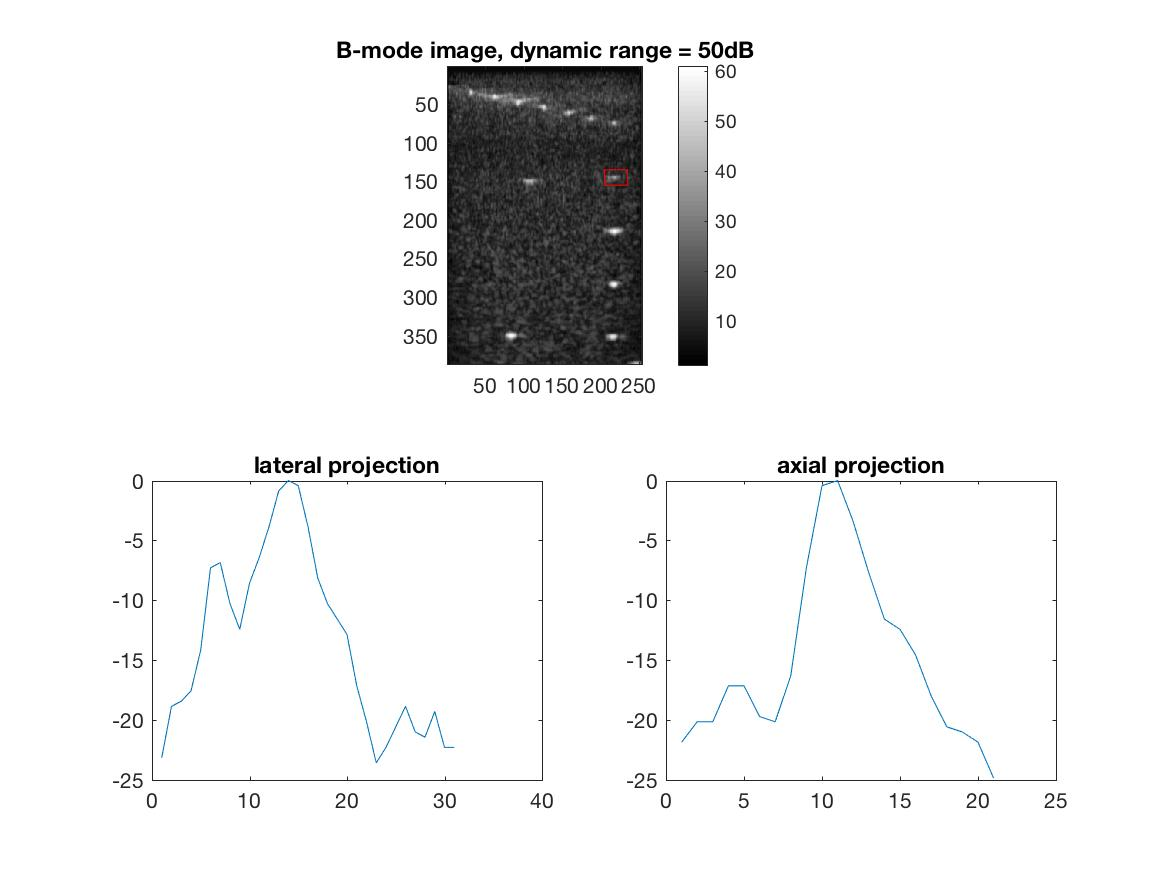
\includegraphics[width=1.0\textwidth]{img_hw1/57-high-pen1.jpg}
    \caption{57-high-pen(In Focus)}
    \label{fig:mesh1}
\end{figure}
\pagebreak
\begin{figure}[h]
    \centering
    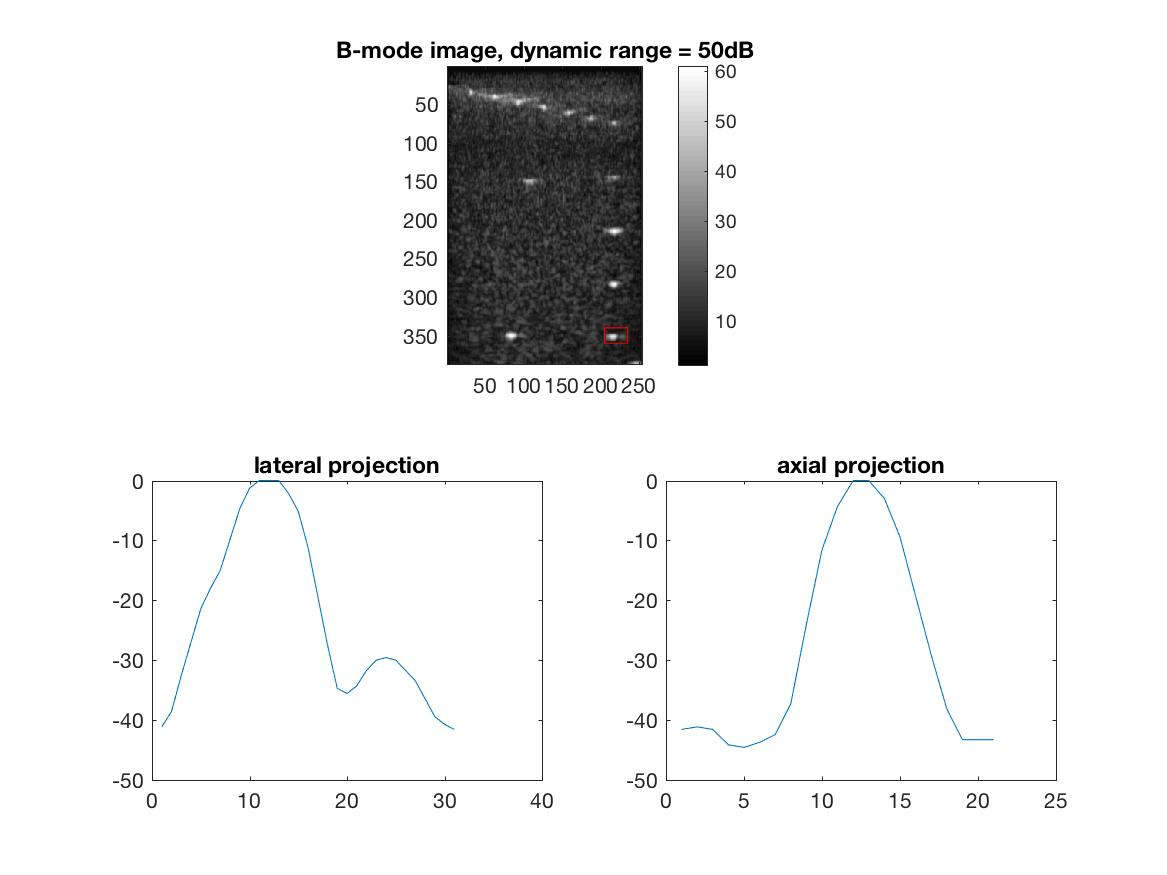
\includegraphics[width=1.0\textwidth]{img_hw1/57-high-pen2.jpg}
    \caption{57-high-pen(Out Focus)}
    \label{fig:mesh1}
\end{figure}
\pagebreak

\item{\emph{5.7cm/high gain/res}}
\begin{center}
\csvautotabular{img_hw1/57-high-res.csv}
\end{center}
\begin{figure}[h]
    \centering
    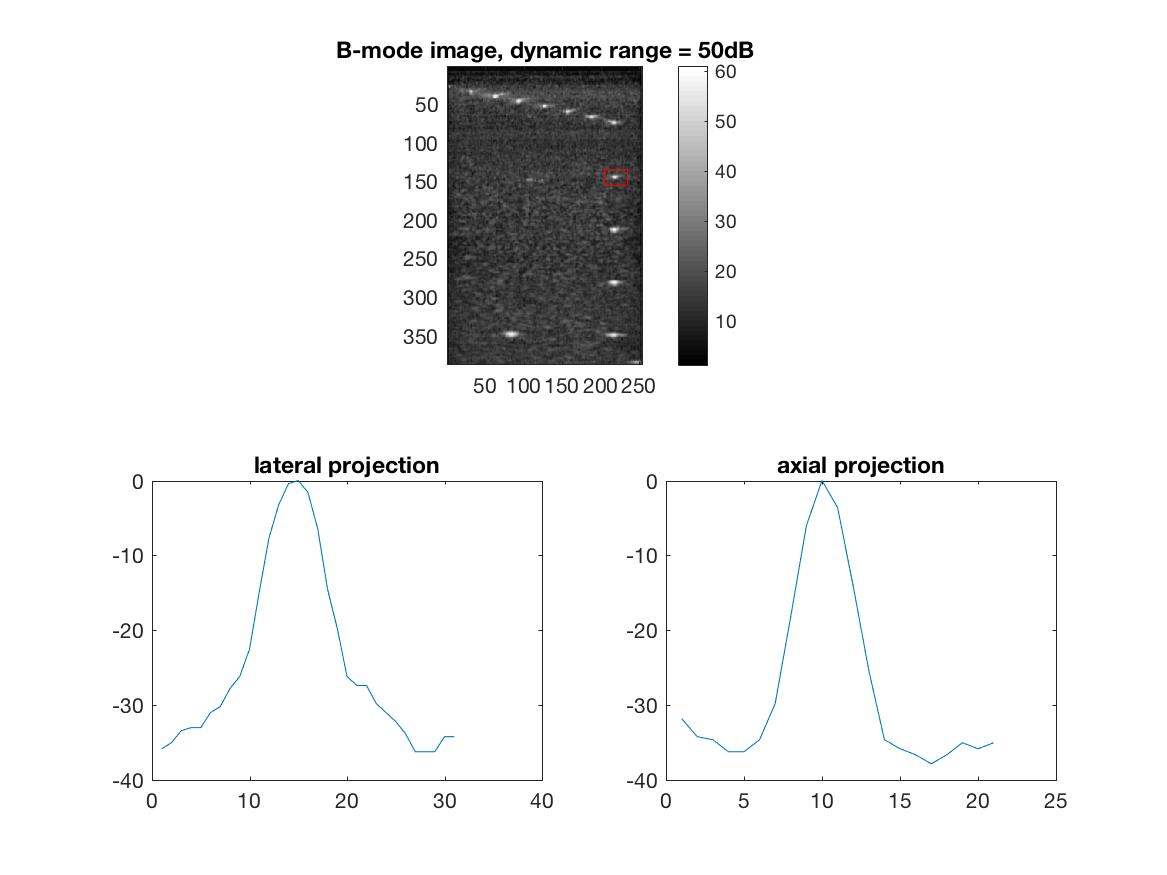
\includegraphics[width=1.0\textwidth]{img_hw1/57-high-res1.jpg}
    \caption{57-high-res(In Focus)}
    \label{fig:mesh1}
\end{figure}
\pagebreak
\begin{figure}[h]
    \centering
    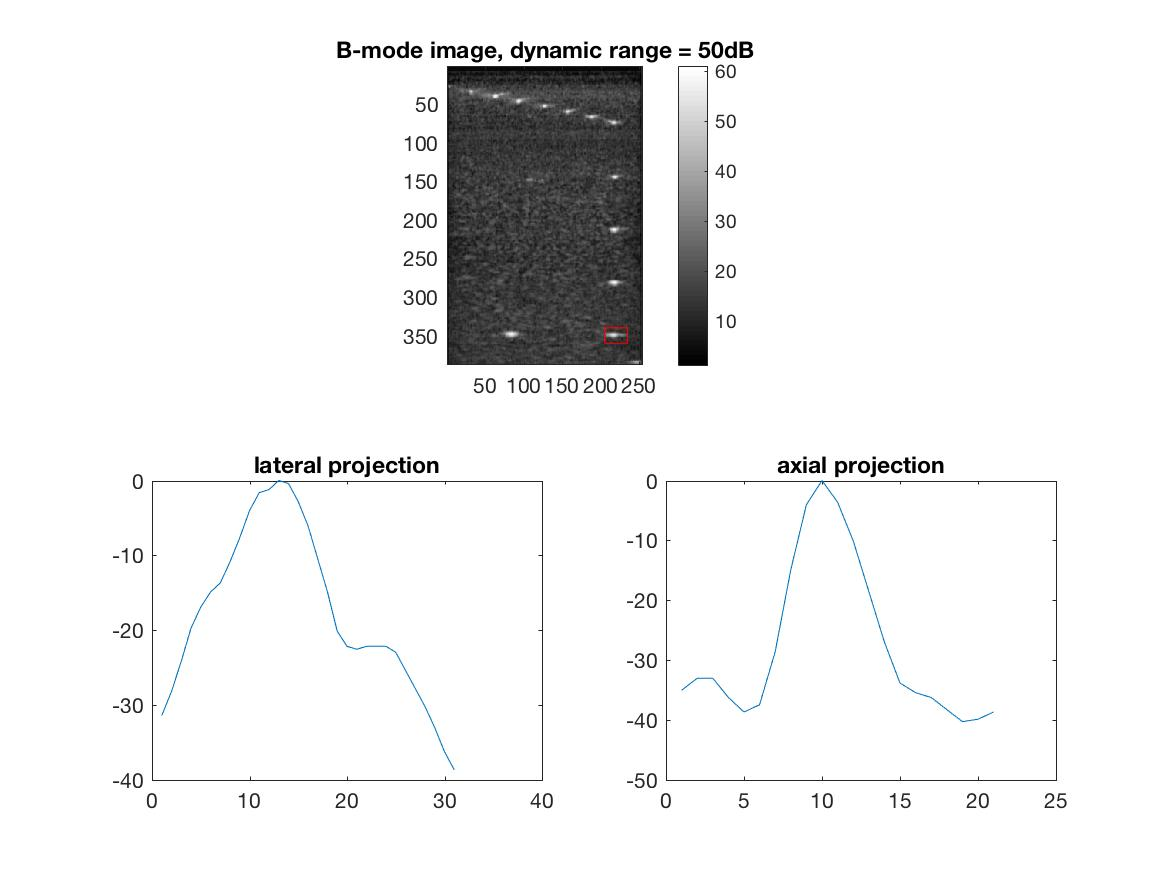
\includegraphics[width=1.0\textwidth]{img_hw1/57-high-res2.jpg}
    \caption{57-high-res(Out Focus)}
    \label{fig:mesh1}
\end{figure}
\pagebreak
\item{\emph{5.7cm/low gain/pen}}
\begin{center}
\csvautotabular{img_hw1/57-low-pen.csv}
\end{center}
\begin{figure}[h]
    \centering
    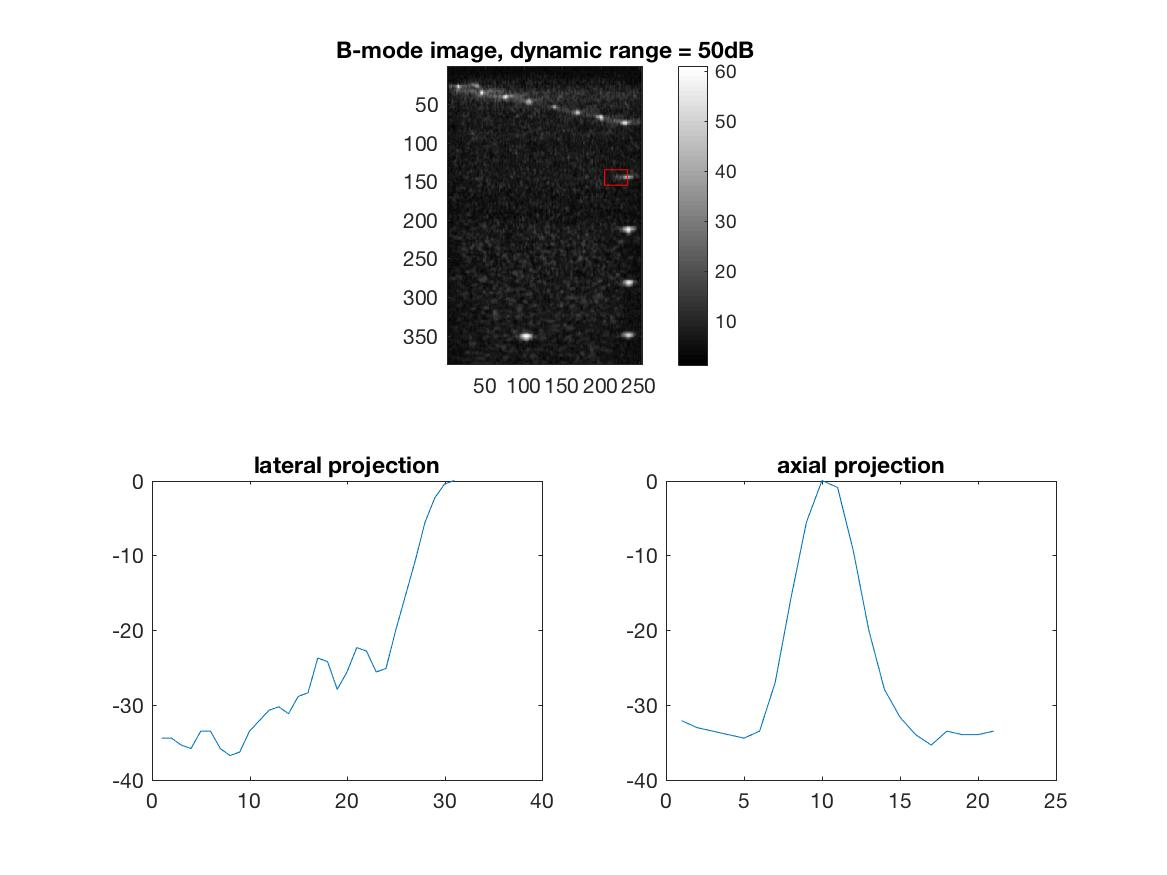
\includegraphics[width=1.0\textwidth]{img_hw1/57-low-pen1.jpg}
    \caption{57-low-pen(In Focus)}
    \label{fig:mesh1}
\end{figure}
\pagebreak
\begin{figure}[h]
    \centering
    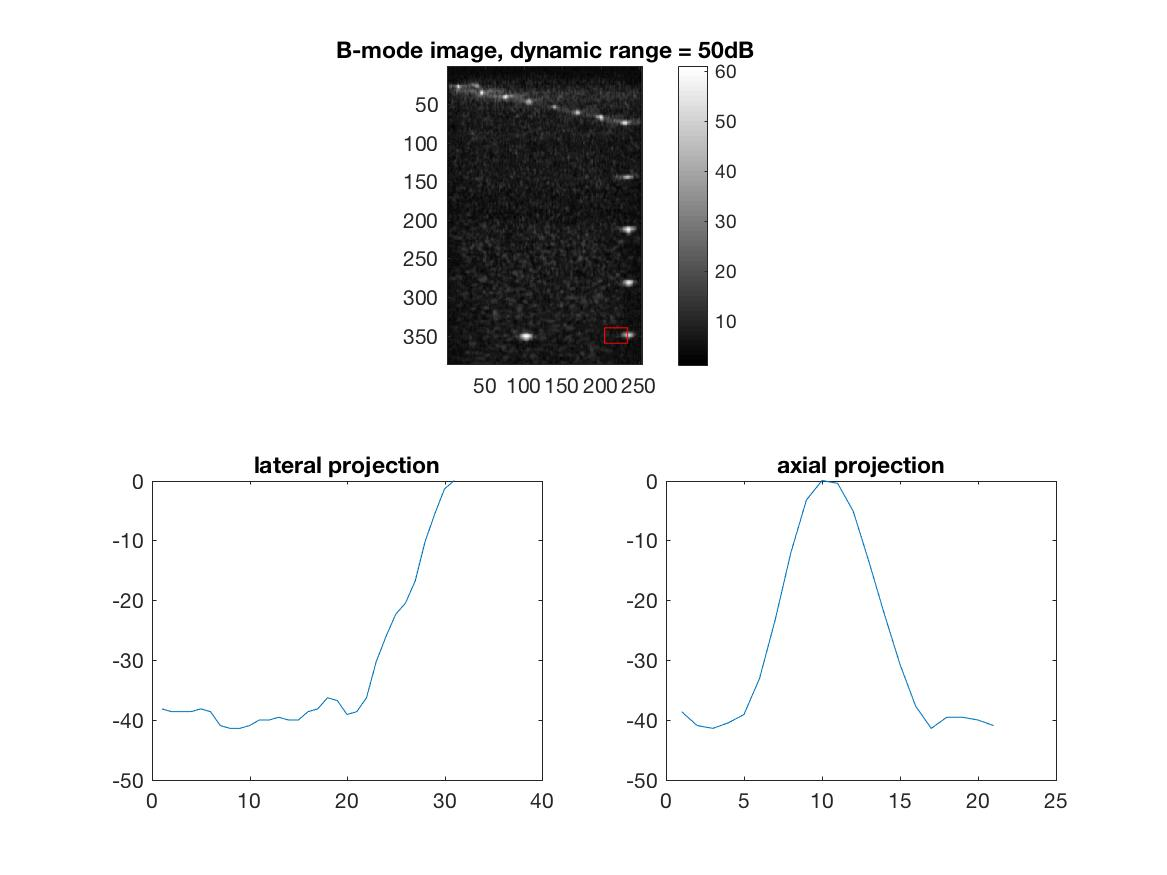
\includegraphics[width=1.0\textwidth]{img_hw1/57-low-pen2.jpg}
    \caption{57-low-pen(Out Focus)}
    \label{fig:mesh1}
\end{figure}
\pagebreak
\item{\emph{5.7cm/low gain/res}}
\begin{center}
\csvautotabular{img_hw1/57-low-res.csv}
\end{center}
\begin{figure}[h]
    \centering
    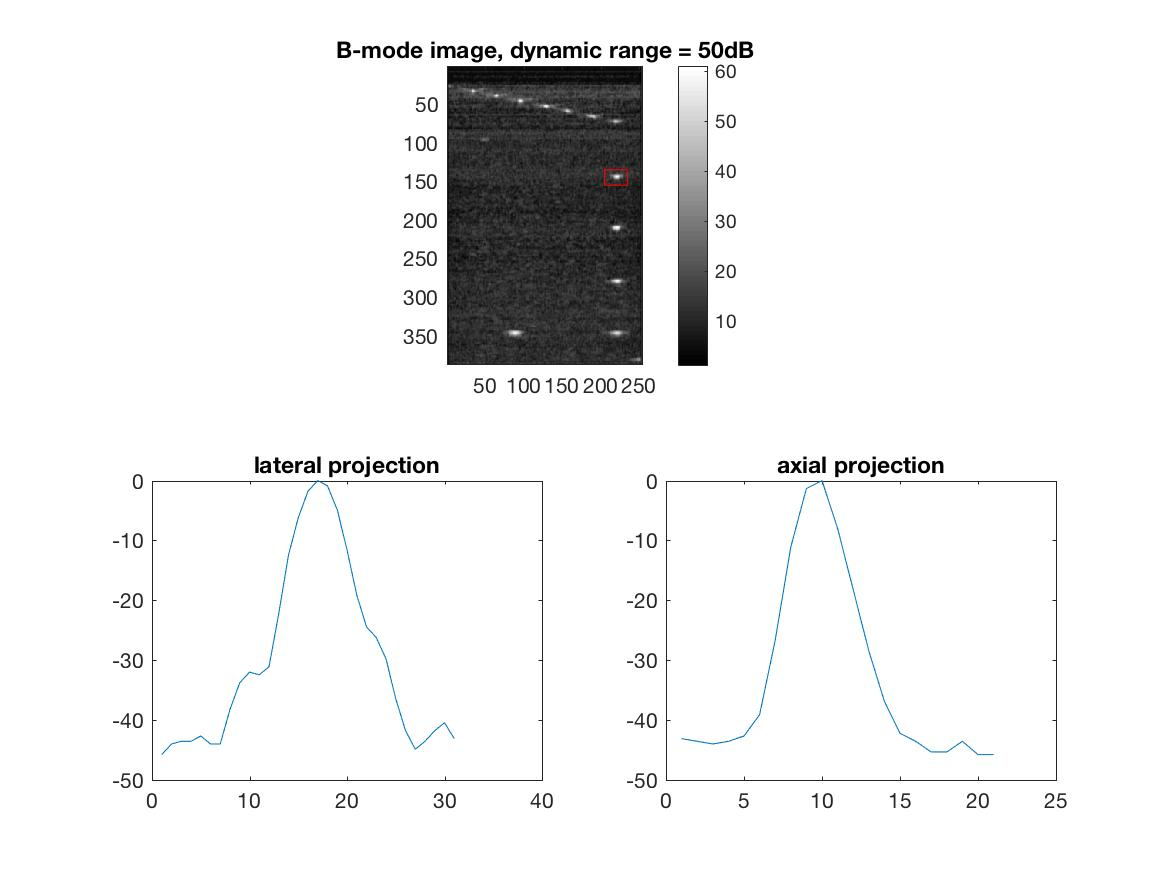
\includegraphics[width=1.0\textwidth]{img_hw1/57-low-res1.jpg}
    \caption{57-low-res(In Focus)}
    \label{fig:mesh1}
\end{figure}
\pagebreak
\begin{figure}[h]
    \centering
    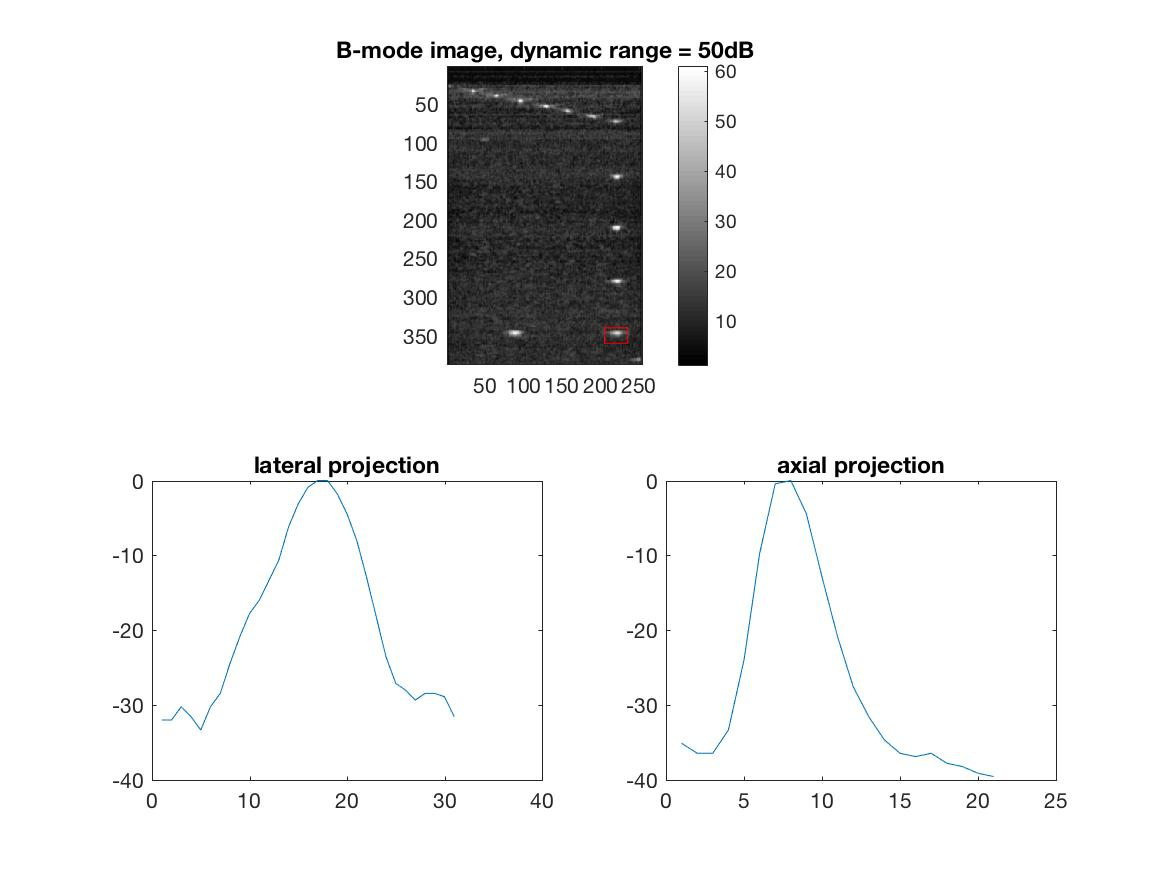
\includegraphics[width=1.0\textwidth]{img_hw1/57-low-res2.jpg}
    \caption{57-low-res(Out Focus)}
    \label{fig:mesh1}
\end{figure}
\pagebreak
\item{\emph{7.1cm/high gain/pen}}
\begin{center}
\csvautotabular{img_hw1/71-high-pen.csv}
\end{center}
\begin{figure}[h]
    \centering
    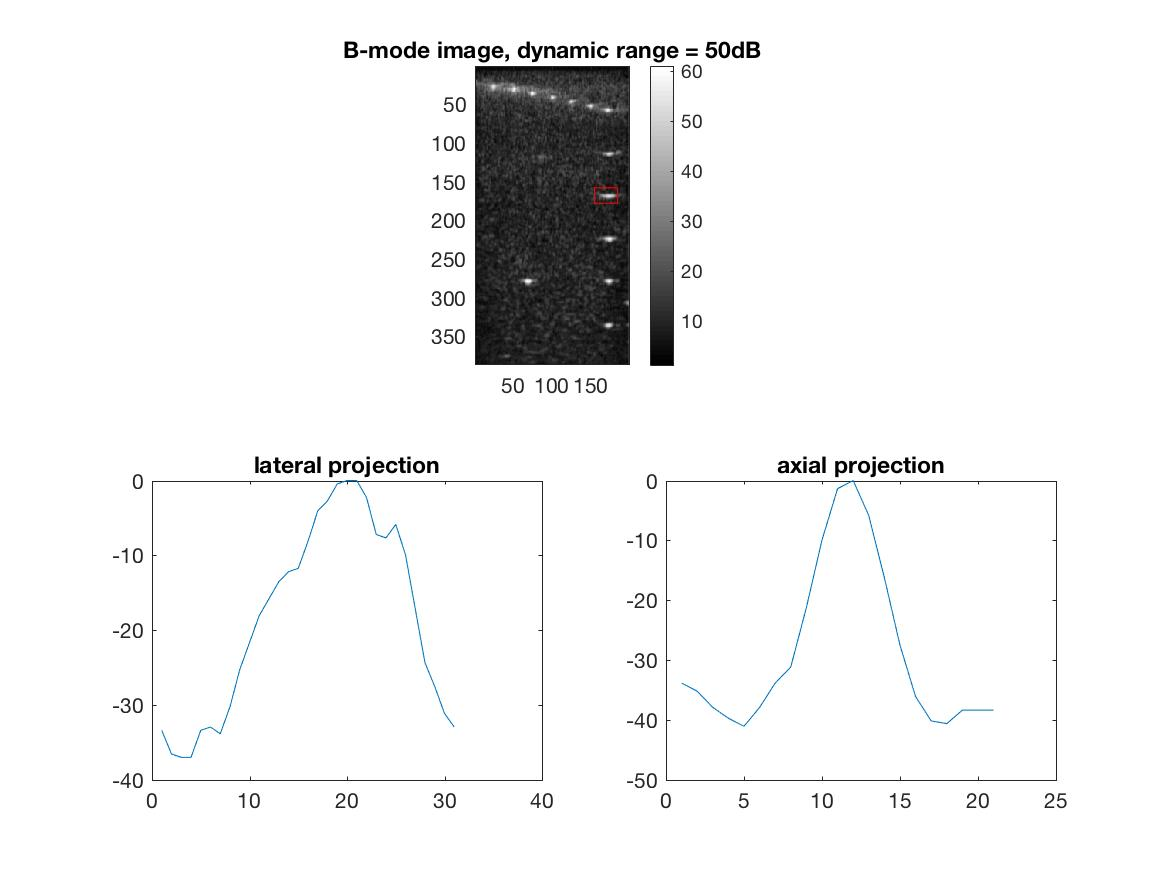
\includegraphics[width=1.0\textwidth]{img_hw1/71-high-pen1.jpg}
    \caption{71-high-pen(In Focus)}
    \label{fig:mesh1}
\end{figure}
\pagebreak
\begin{figure}[h]
    \centering
    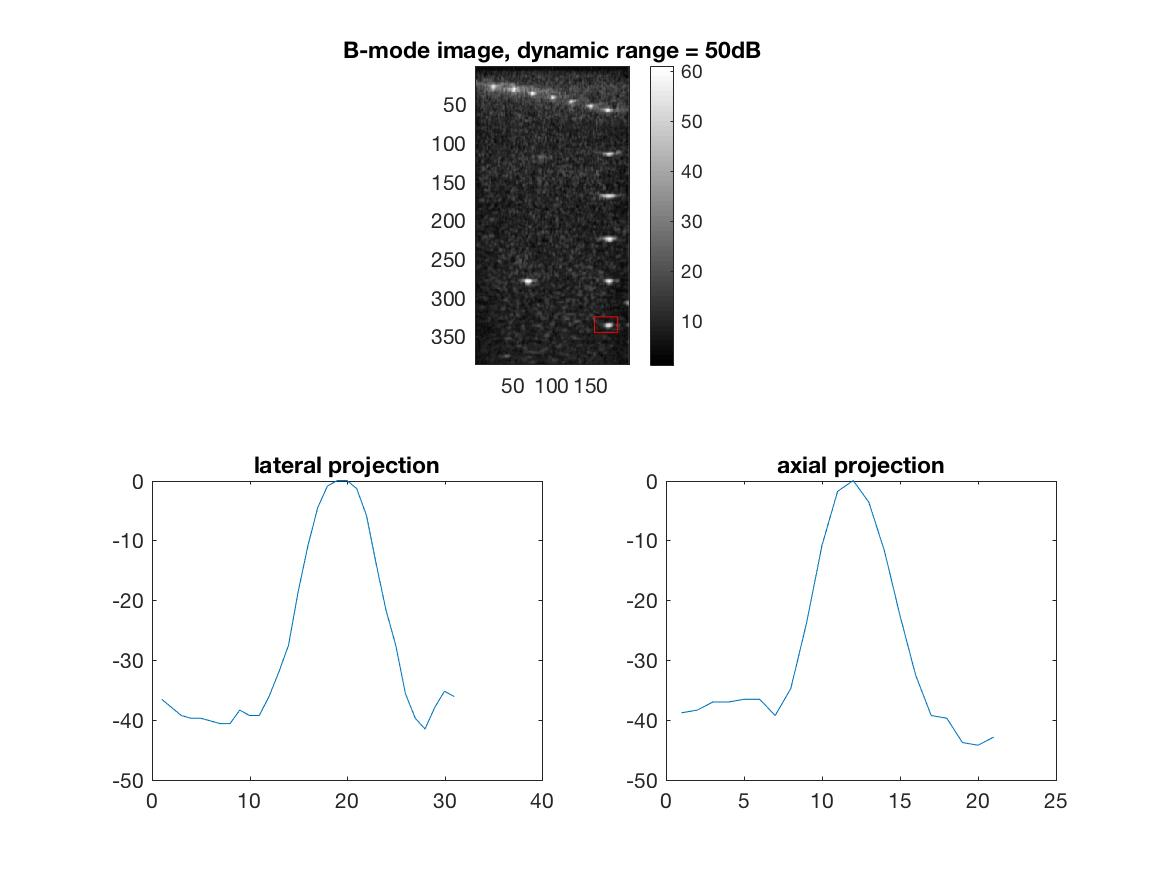
\includegraphics[width=1.0\textwidth]{img_hw1/71-high-pen2.jpg}
    \caption{71-high-pen(Out Focus)}
    \label{fig:mesh1}
\end{figure}
\pagebreak
\item{\emph{7.1cm/high gain/res}}
\begin{center}
\csvautotabular{img_hw1/71-high-res.csv}
\end{center}
\begin{figure}[h]
    \centering
    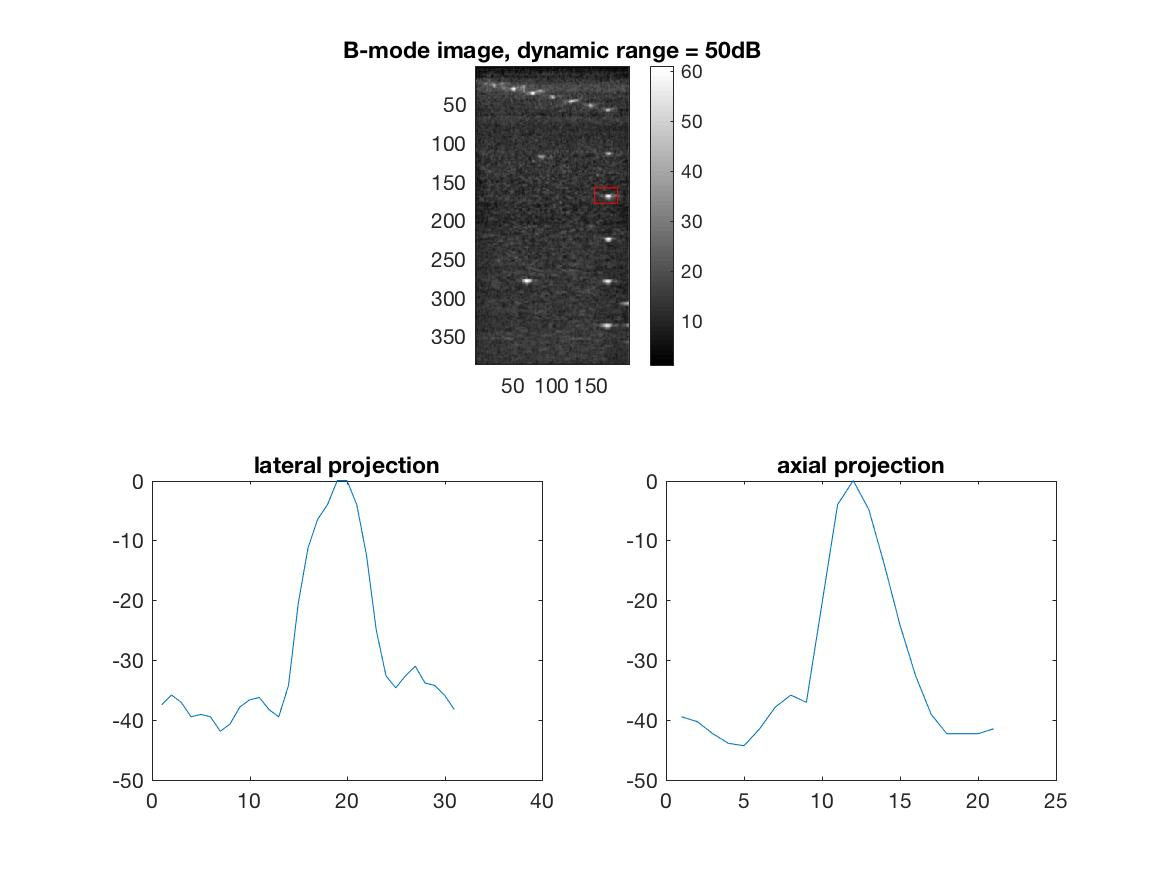
\includegraphics[width=1.0\textwidth]{img_hw1/71-high-res1.jpg}
    \caption{71-high-res(In Focus)}
    \label{fig:mesh1}
\end{figure}
\pagebreak
\begin{figure}[h]
    \centering
    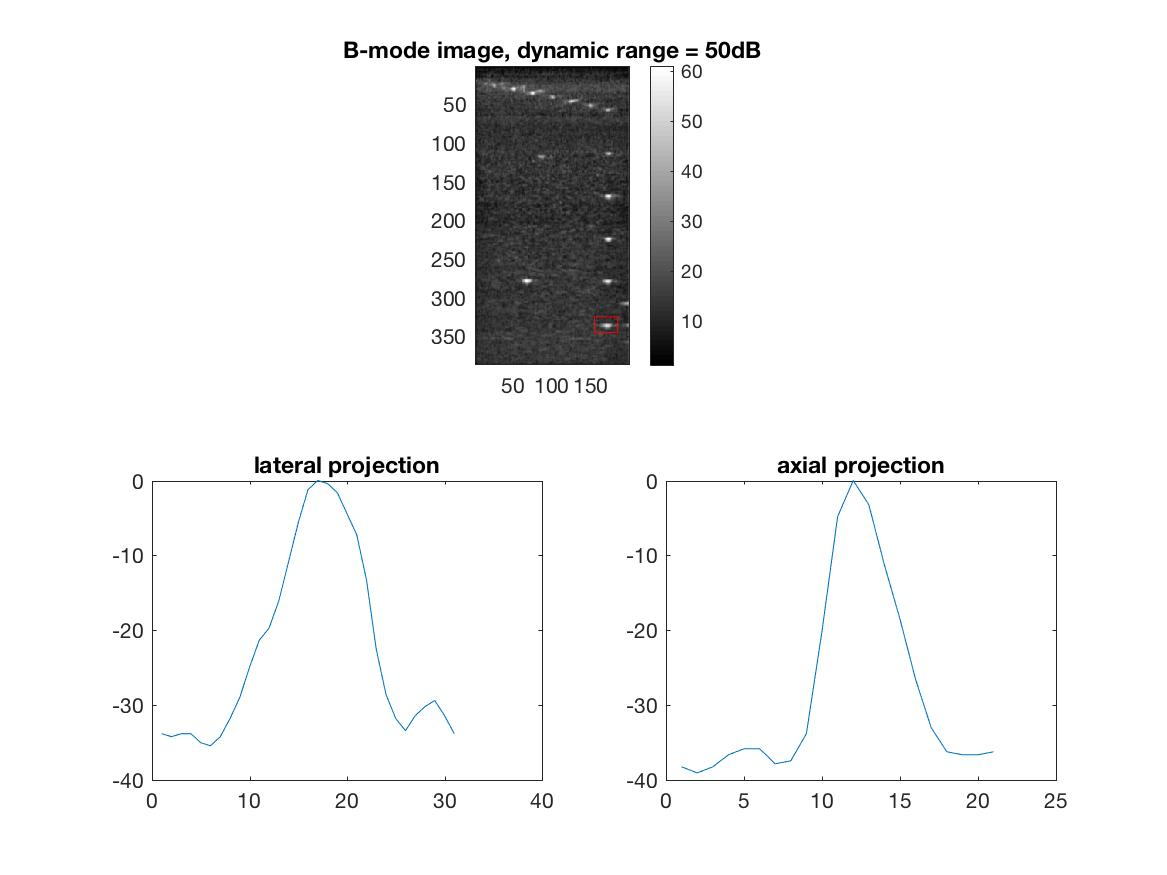
\includegraphics[width=1.0\textwidth]{img_hw1/71-high-res2.jpg}
    \caption{71-high-res(Out Focus)}
    \label{fig:mesh1}
\end{figure}
\pagebreak
\item{\emph{7.1cm/low gain/pen}}
\begin{center}
\csvautotabular{img_hw1/71-low-pen.csv}
\end{center}
\begin{figure}[h]
    \centering
    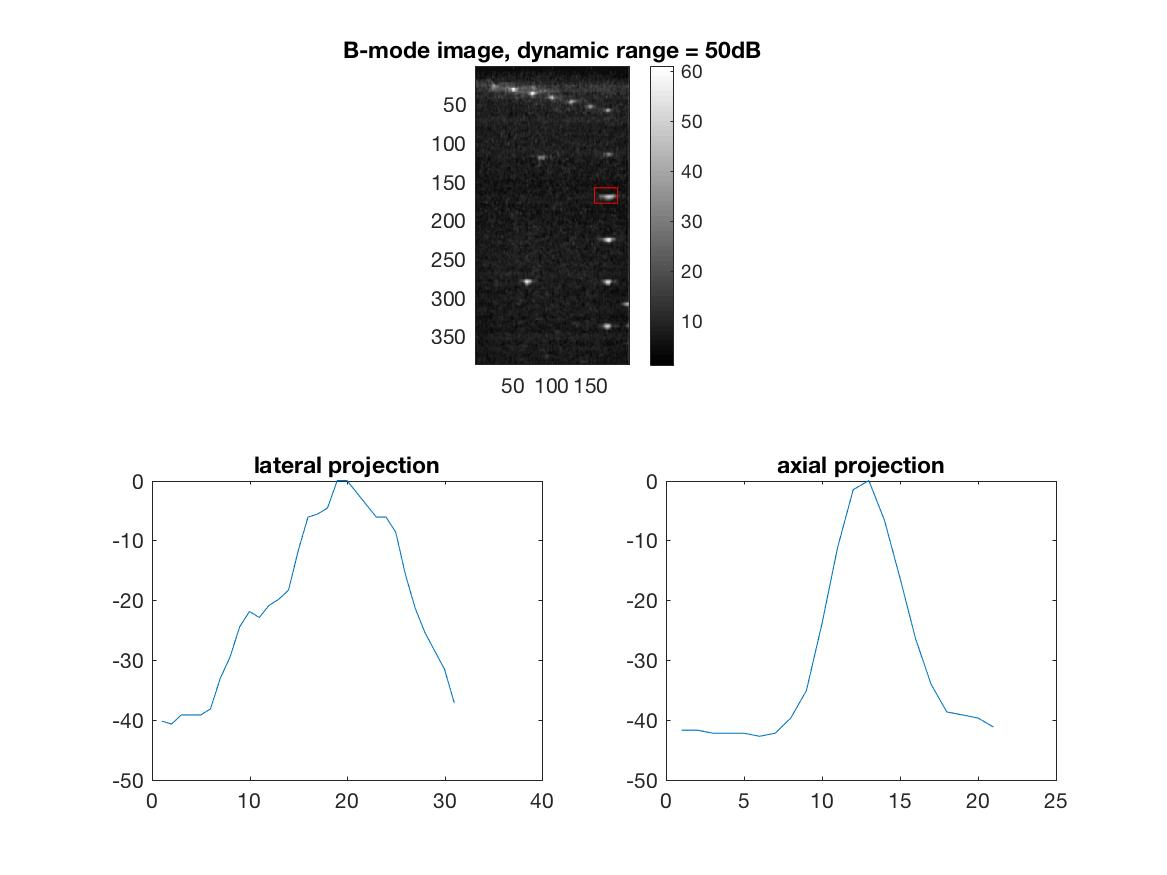
\includegraphics[width=1.0\textwidth]{img_hw1/71-low-pen1.jpg}
    \caption{71-low-pen(In Focus)}
    \label{fig:mesh1}
\end{figure}
\pagebreak
\begin{figure}[h]
    \centering
    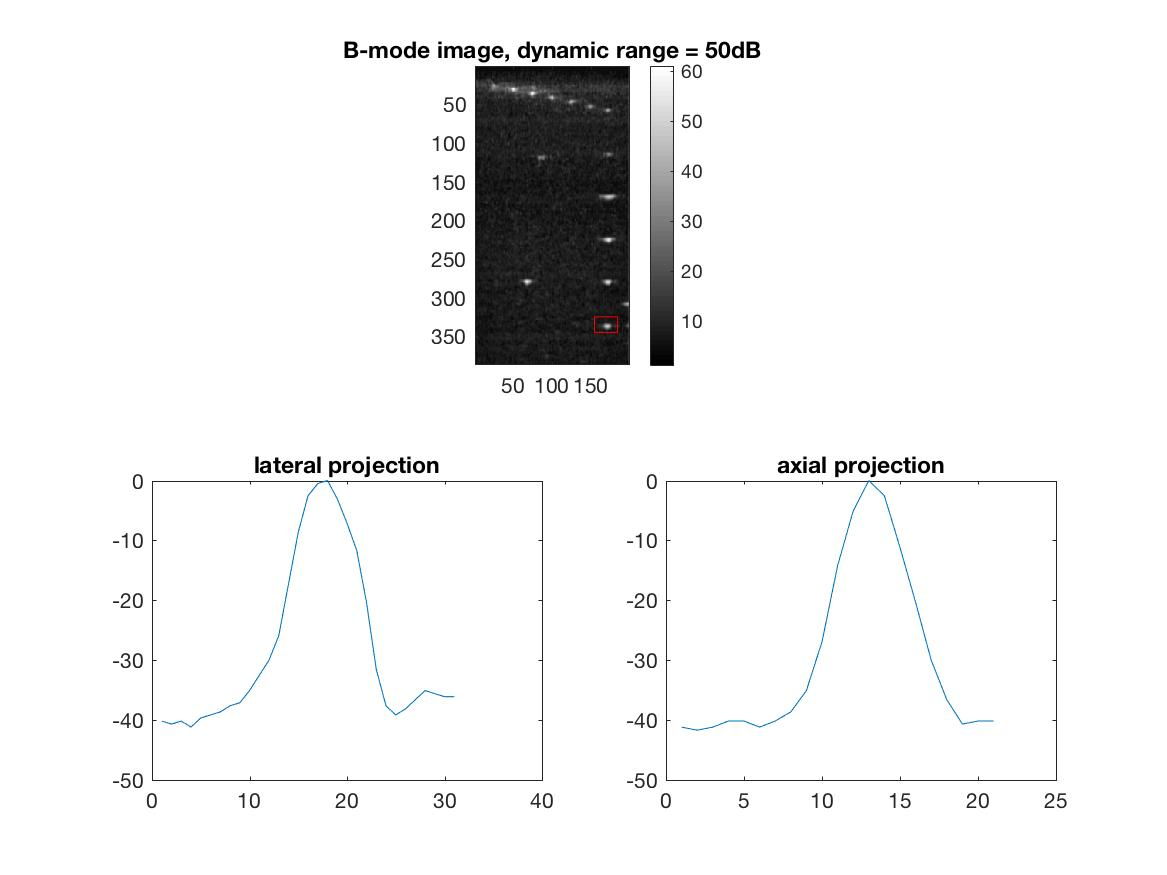
\includegraphics[width=1.0\textwidth]{img_hw1/71-low-pen2.jpg}
    \caption{71-low-pen(Out Focus)}
    \label{fig:mesh1}
\end{figure}
\pagebreak
\item{\emph{7.1cm/low gain/res}}
\begin{center}
\csvautotabular{img_hw1/71-low-res.csv}
\end{center}
\begin{figure}[h]
    \centering
    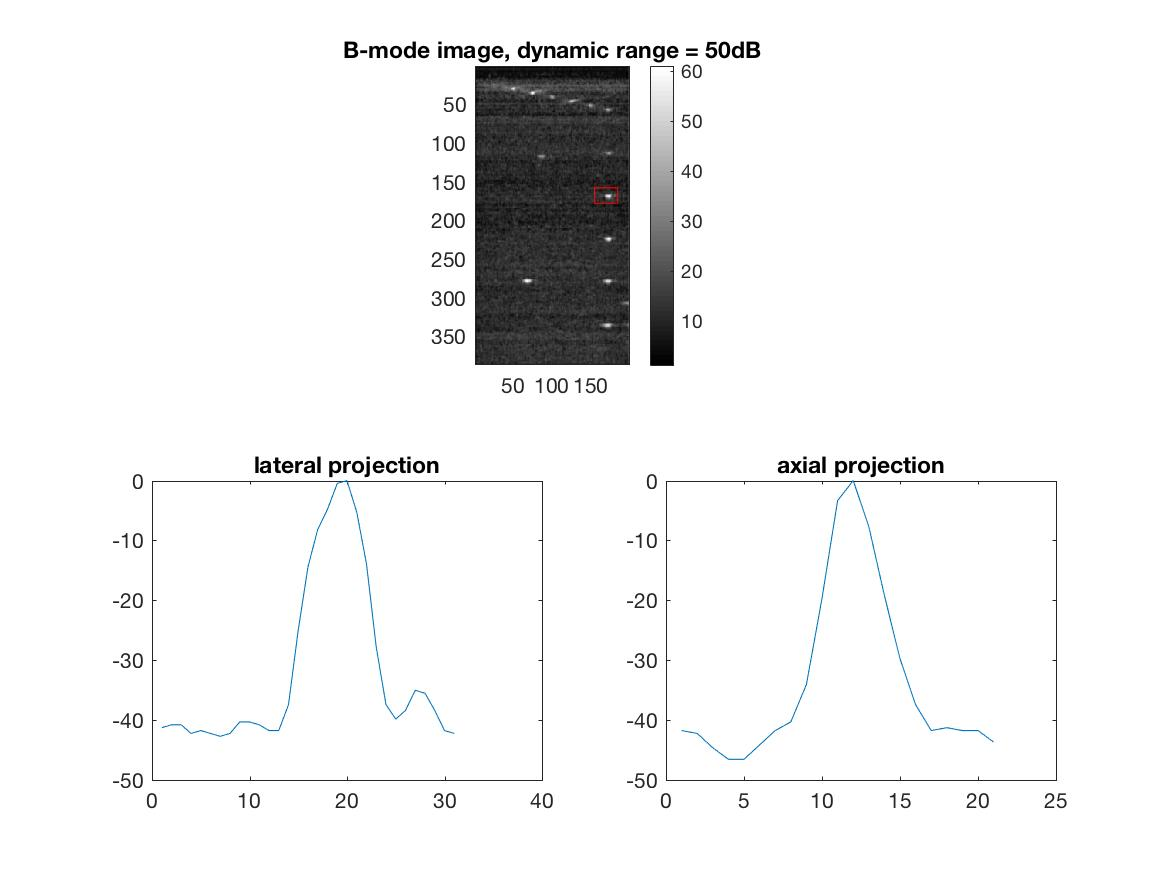
\includegraphics[width=1.0\textwidth]{img_hw1/71-low-res1.jpg}
    \caption{71-low-res(In Focus)}
    \label{fig:mesh1}
\end{figure}
\pagebreak
\begin{figure}[h]
    \centering
    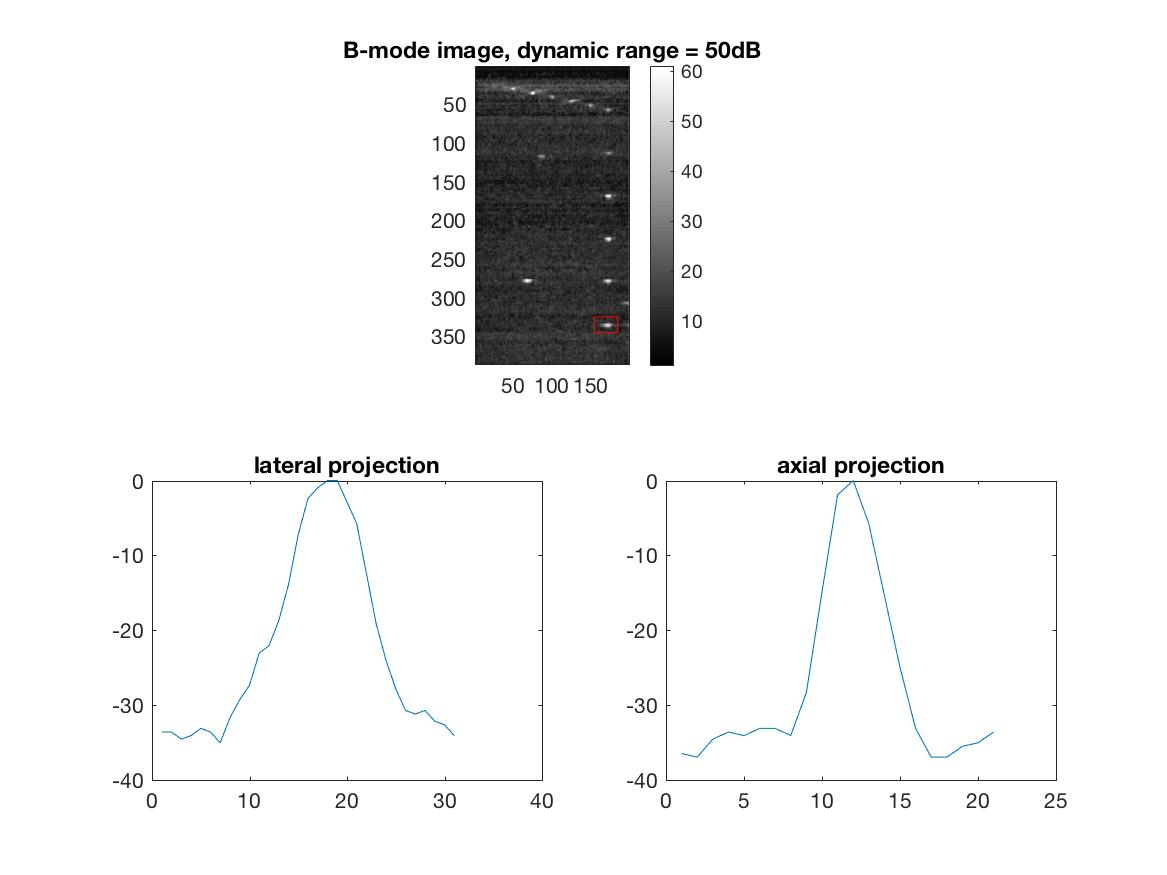
\includegraphics[width=1.0\textwidth]{img_hw1/71-low-res2.jpg}
    \caption{71-low-res(Out Focus)}
    \label{fig:mesh1}
\end{figure}
\pagebreak

\end{itemize}
\end{document}
